\begin{itemize}
\item L'un des inconvénients du crible d’Ératosthène est que lors de l'initialisation, on stocke les nombres de 1 à une limite n, définie arbitrairement, dans une liste, ce qui peut prendre beaucoup de place en mémoire si la limite est élevée. On ne peut donc pas traiter une grande liste si on a pas suffisamment de place en mémoire.\\

\item Pour commencer à traiter une liste, il faut forcément commencer à 2 car on retire les multiples de chaque nombre traité de la liste. Donc on ne peut pas commencer à un nombre strictement supérieur à 2 si on ne veut pas oublier les multiples de 2.\\
Cela implique que si on veut arrêter le programme, il faut sauvegarder l'état courant, ce qui prend un peu plus de place en mémoire.\\

\item Contrairement au petit théorème de Fermat, qui lui teste les nombres de façon indépendante, le crible d’Ératosthène n'est pas parallélisable car on enlève les multiples du nombre que l'on traite dans la même liste, deux threads ou processus ne peuvent donc pas accéder à cette liste en simultané. Donc on traite moins de nombres à la fois.\\
\end{itemize}

Sur les screens suivants, on peut voir la différence de temps que mettent le crible d’Ératosthène (premier screen) et le petit théorème de Fermat (second screen) pour générer une liste de nombres premiers allant de 3 à 1 000 000.\\

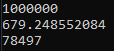
\includegraphics[scale=1]{images/eratosthene_1000000.png}
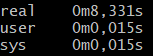
\includegraphics[scale=1]{images/comp_fermat.png}\\
Sur la première image, réalisé à partir du crible d'ératosthène, pour chercher les nombres premiers entre 2 à 1 000 000 on met 679s ce qui équivaut à 11 min et on a trouvé 78497 nombres premiers.\\
